
\begin{frame}{Componente SeekBar en Android}
\textbf{¿Qué es un SeekBar?}

\begin{itemize}
    \item Es un componente de interfaz gráfica que permite al usuario seleccionar un valor dentro de un rango deslizando un control horizontal.
    \item Es una extensión de la clase ProgressBar con interacción del usuario.
\end{itemize}

\vspace{0.5cm}

\textbf{¿Para qué sirve?}
\begin{itemize}
    \item Ajustar valores continuos o discretos (ej. volumen, brillo, progreso).
    \item Permitir entrada intuitiva mediante deslizamiento.
    \item Controlar parámetros en tiempo real.
\end{itemize}

\vspace{0.5cm}

\textbf{Características principales:}
\begin{itemize}
    \item Permite definir valores mínimo, máximo y progreso actual.
    \item Puede escuchar cambios mediante un listener (OnSeekBarChangeListener).
    \item Es altamente personalizable (colores, tamaño, estilo).
\end{itemize}


\end{frame}


\begin{frame}[fragile]
\frametitle{Demo 08: Agregar SeekBars}
\begin{columns}
\column{0.80\linewidth}
Del Repositorio Github:
\begin{itemize}
\item Copiar el archivo MainActivity\_Demo08.java (dentro del Folder códigosJAVA) al mismo directorio donde esta el MainActivity.java
\item Copiar el archivo activity\_main\_demo08.xml (dentro del Folder Carpeta\_layout) al mismo directorio donde esta el activity\_main.xml
%\item Copiar los archivos \textit{cgup.jpg} y \textit{logo\_upv\_2019.png} localizados dentro de la folder \textit{Carpeta\_drawable} en el directorio \textit{res/drawable} del proyecto de AS.
\item Modificar en el archivo AndroidManifest.xml la cadena \textit{.MainActivity\_Demo07} por \textit{.MainActivity\_Demo08}
\end{itemize}

\begin{block}{Demo \#08}
Muestra una App dos SeekBars (la segunda utiliza separadores finitos). La primera SeekBar actualiza el contenido de TextView conforme la seleccion del usuario. 
\end{block}


\column{0.20\linewidth}

\begin{center}
 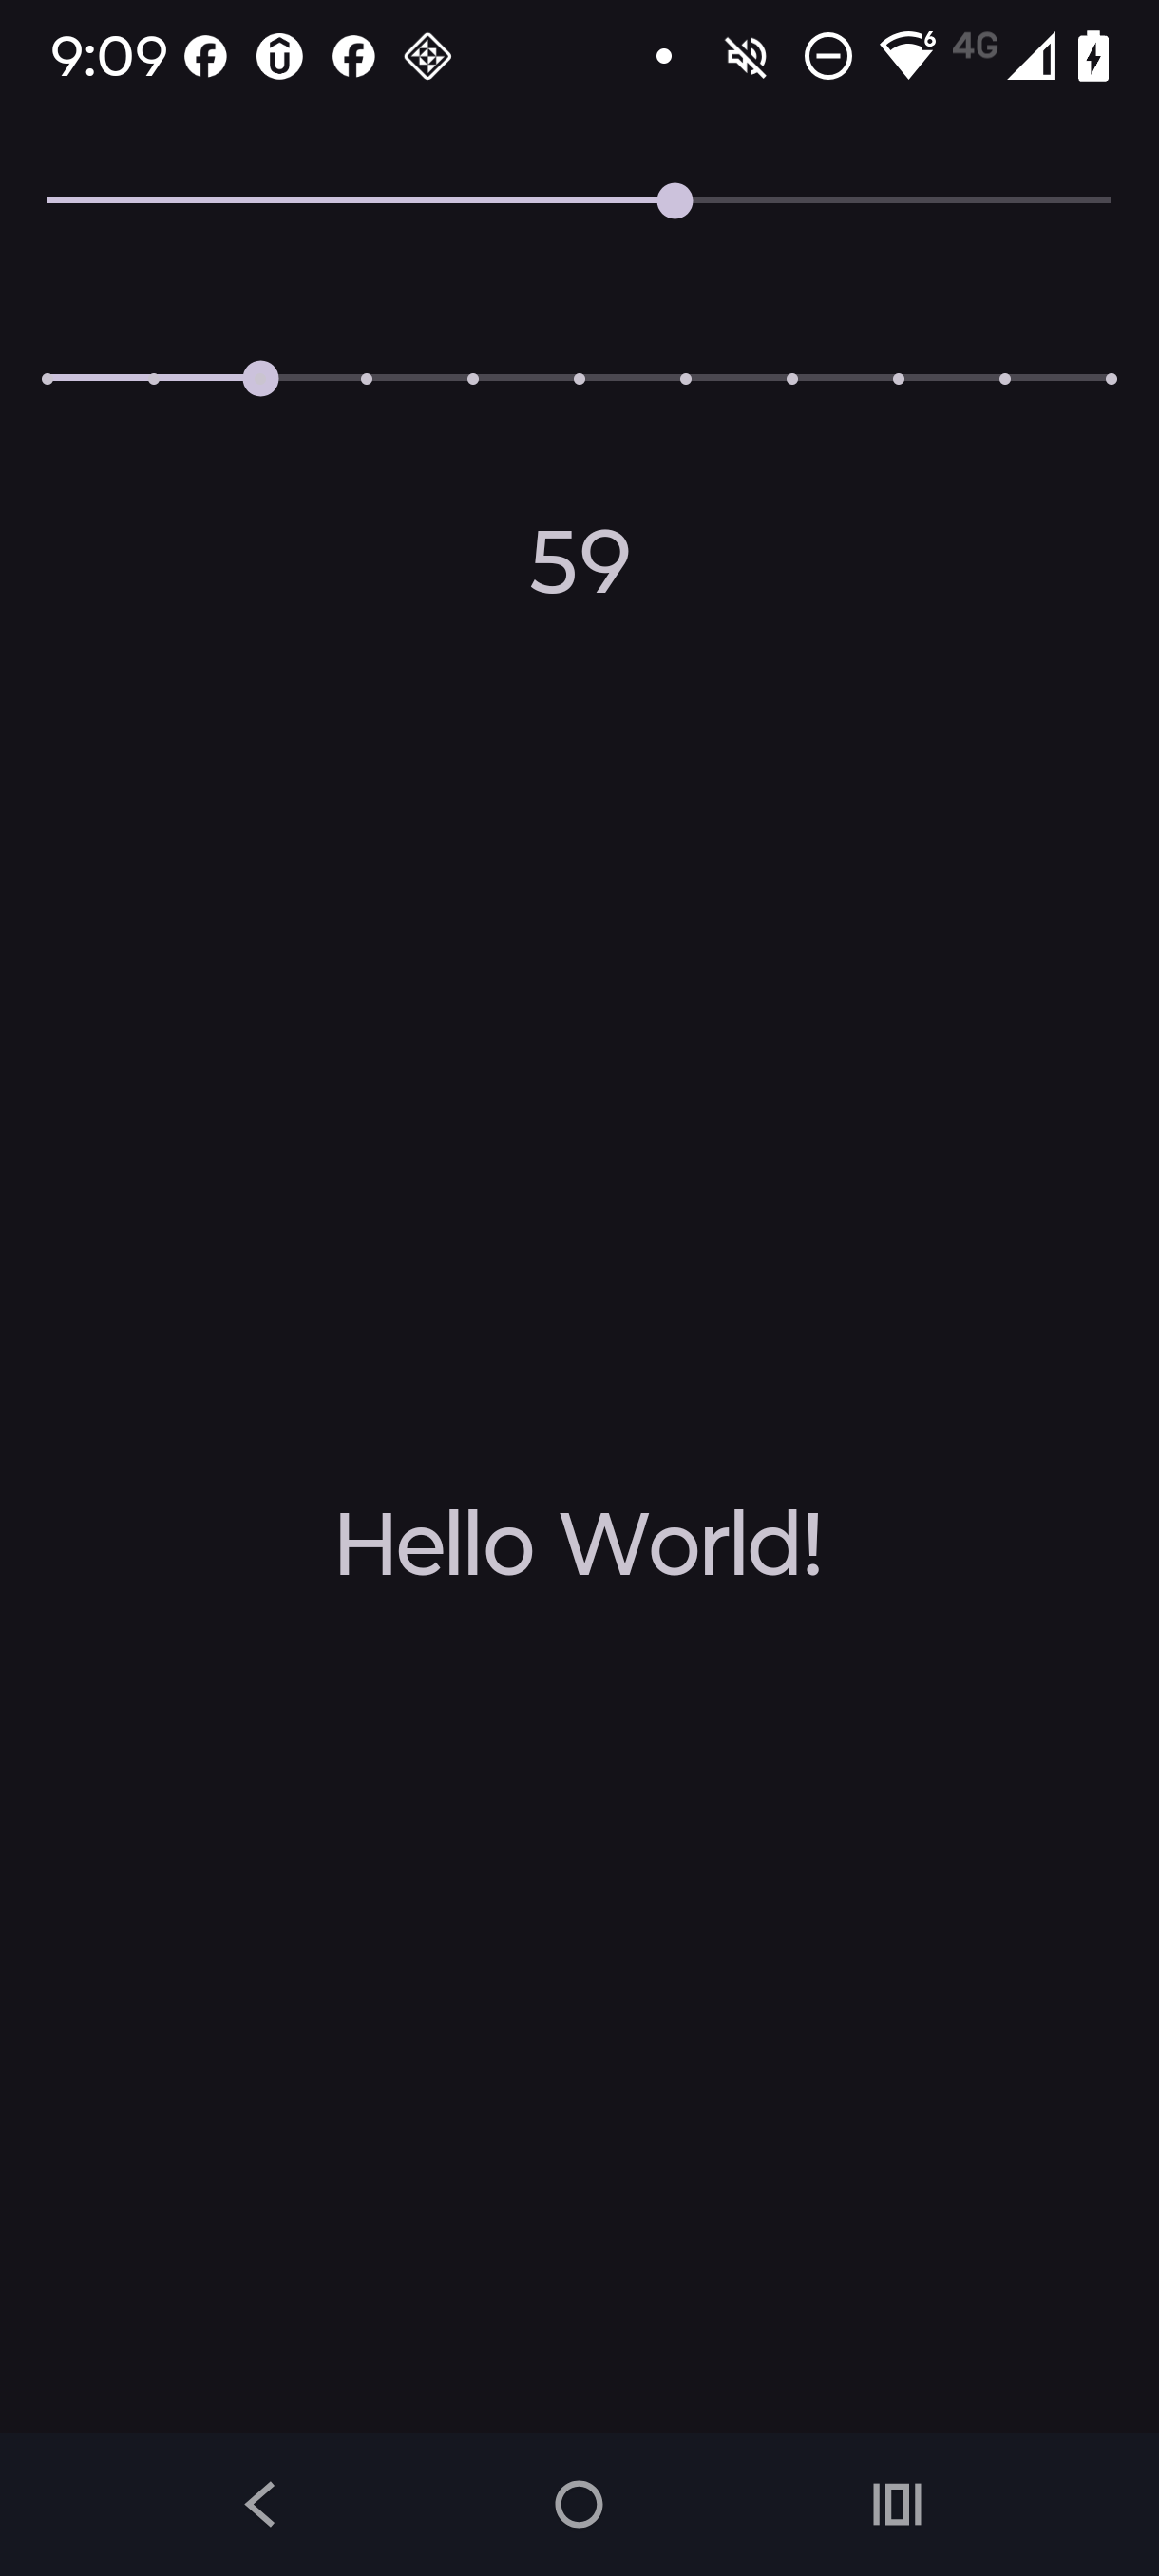
\includegraphics[width=0.98\textwidth]{02_TallerCBTis/figs/Demo08}
\end{center}

\end{columns}

\end{frame}



%\begin{frame}{startActivityForResult y onActivityResult}


\begin{frame}[fragile]
\frametitle{startActivityForResult y onActivityResult}  
\textbf{¿Para qué sirven?}

\begin{itemize}
    \item Permiten iniciar una actividad esperando un resultado de regreso.
    \item Son útiles cuando se necesita que una segunda pantalla devuelva información (por ejemplo, selección de datos o confirmaciones).
\end{itemize}

\vspace{0.4cm}

\textbf{Flujo de funcionamiento:}
\begin{enumerate}
    \item Se inicia la actividad con \texttt{startActivityForResult()}.
    \item La segunda actividad procesa la información.
    \item Se devuelve un resultado mediante \texttt{setResult()}.
    \item La actividad original recibe el resultado en \texttt{onActivityResult()}.
\end{enumerate}


\textbf{Ejemplo en Java:}
\begin{block}{}
\small
\begin{minted}[linenos,fontsize=\tiny]{java}
// Lanzar actividad
Intent intent = new Intent(this, SegundaActivity.class);
startActivityForResult(intent, 1);

// Recibir resultado
@Override
protected void onActivityResult(int requestCode, int resultCode, Intent data) {
    if (requestCode == 1 && resultCode == RESULT_OK) {
        String resultado = data.getStringExtra("dato");
    }
}
\end{minted}
\end{block}

\end{frame}




\begin{frame}[fragile]
\frametitle{Demo 09: Lectura y Escritura de Archivos de Texto}
\begin{columns}
\column{0.80\linewidth}
Del Repositorio Github:
\begin{itemize}
\item Copiar el archivo \textit{MainActivity\_Demo09.java} (dentro del Folder códigosJAVA) al mismo directorio donde esta el MainActivity.java
\item Copiar el archivo \textit{activity\_main\_demo09.xml} (dentro del Folder Carpeta\_layout) al mismo directorio donde esta el activity\_main.xml

%\item Copiar los archivos \textit{cgup.jpg} y \textit{logo\_upv\_2019.png} localizados dentro de la folder \textit{Carpeta\_drawable} en el directorio \textit{res/drawable} del proyecto de AS.
\item Modificar en el archivo \textit{AndroidManifest.xml} la cadena \textit{.MainActivity\_Demo08} por \textit{.MainActivity\_Demo09}.
\item Ir a la linea 22 de archivo del archivo \textit{MainActivity\_Demo09.java}, poner el cursos en la palabra (en Rojo) \textit{documentfile}, presionar la combinación ALT+ENTER, y seleccionar de la lista desplegable la opcion ``Add dependency on ....''. Esto quitará el error y hara los ajustes necesarios. 
\end{itemize}

%\begin{block}{Demo \#09}
%Un App que permite escribir el contenido de un EditText a un archivo y cargar el contenido de cualquier archivo en el EditText
%\end{block}


\column{0.20\linewidth}

\begin{center}
 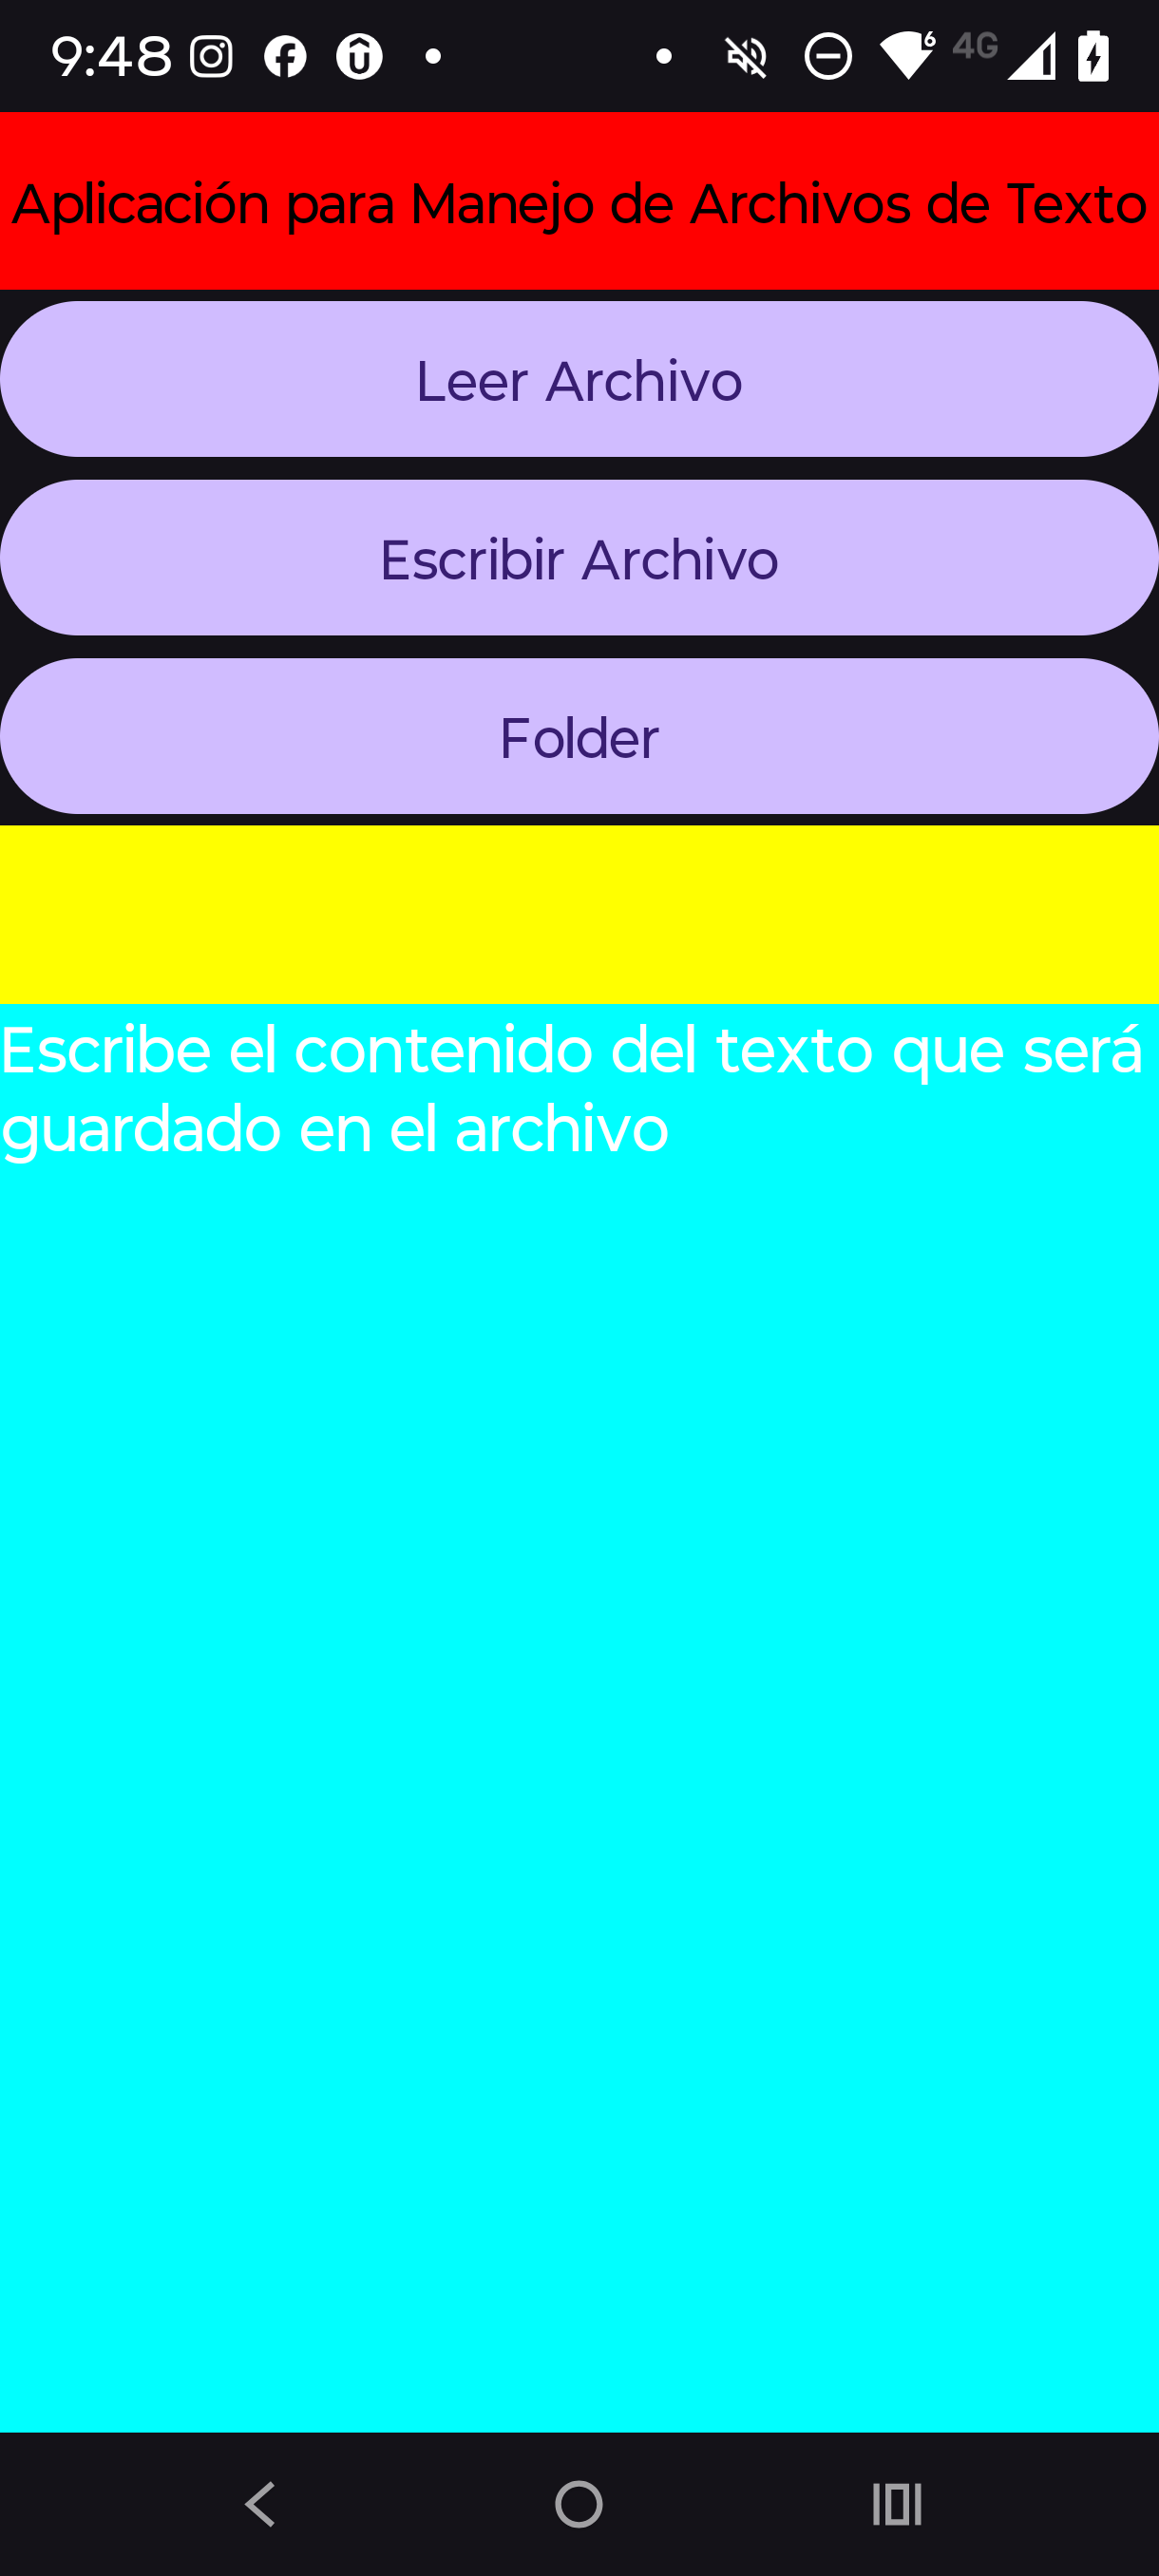
\includegraphics[width=0.98\textwidth]{02_TallerCBTis/figs/Demo09}
\end{center}

\end{columns}

\end{frame}

